\documentclass[14pt]{extarticle}
 
\usepackage[bottom=1cm,right=1cm,left=2cm]{geometry}
\usepackage{graphicx}
 
%Russian-specific packages
%--------------------------------------
\usepackage[T2A,T1]{fontenc}
\usepackage[utf8]{inputenc}
\usepackage[english,russian]{babel}
\usepackage{amsmath}
\usepackage{booktabs}
\usepackage{caption}
\usepackage{float}
\usepackage{array}
\usepackage{geometry}
\usepackage{adjustbox}
\usepackage{tocloft} % Для настройки оглавления
\usepackage{hyperref} % Для гиперссылок
\geometry{a4paper, left=30mm, right=15mm, top=20mm, bottom=20mm}
%--------------------------------------
\usepackage{amsfonts}
 

\setlength{\topmargin}{-2cm}
\renewcommand{\baselinestretch}{1.5} % Межстрочный интервал 1.5
\setlength{\parindent}{1.25cm} % Абзацный отступ 1.25 см
\setlength{\cftbeforesecskip}{5pt} % Отступы в оглавлении

\begin{document}
 
\pagenumbering{gobble}
 
\begin{titlepage}
\fontsize{14pt}{14pt}\selectfont
\newcommand{\HRule}{\rule{\linewidth}{0.5mm}}

\center

\textsc{ФЕДЕРАЛЬНОЕ ГОСУДАРСТВЕННОЕ АВТОНОМНОЕ}\\
\textsc{ОБРАЗОВАТЕЛЬНОЕ УЧРЕЖДЕНИЕ ВЫСШЕГО ОБРАЗОВАНИЯ}\\
\textsc{«НАЦИОНАЛЬНЫЙ ИССЛЕДОВАТЕЛЬСКИЙ УНИВЕРСИТЕТ}\\
\textsc{«ВЫСШАЯ ШКОЛА ЭКОНОМИКИ»}\\
\textsc{\bfseries Московский институт электроники и математики}\\[1.5cm]

\textsc{Долгополова Анна Руслановна}\\
\textsc{\large\bfseries Анализ датасетов на объем избыточной памяти}\\[2cm]

\vfill
\textsc{Проектная работа}
\textsc{студента образовательной программы бакалавриата}\\
\textsc{«Прикладная математика»}\\
\textsc{по направлению подготовки 01.03.04 ПРИКЛАДНАЯ МАТЕМАТИКА}\\[1.5cm]

\begin{flushright}
Студент\\
А. Р. Долгополова
\end{flushright}

\hfill
\begin{minipage}{0.45\textwidth}
    \begin{tabular}{p{\textwidth}}
    \begin{flushright}
    Руководитель ПР\\
    Ученая степень, должность\\
    И.О. Фамилия\\[0.5cm]
    \end{flushright}
    \end{tabular}
\end{minipage}% 

\vfill
{\large\bfseries Москва \the\year г.}

\end{titlepage}

% Оглавление
\tableofcontents
\newpage

% Упоминание об использовании ИИ
\section*{Использование генеративных нейросетей}
При подготовке данного отчёта использовалась генеративная нейросеть DeepSeek для оптимизации формулировок и структуры документа. Все технические расчёты, анализ данных и выводы выполнены автором самостоятельно.

\section{Аннотация}

В данной работе исследуется эффективность применения метода главных компонент (PCA) для сжатия изображений. Проведён анализ изображений различных классов, выявлено, что среднее оптимальное количество используемых главных компонент для класса, что видно на Рис.~\ref{fig:components_class}, варьируется от 23 до 71, также исходя из данных, представленных на Рис.~\ref{fig:components_image}, в классе наблюдается дисперсия оптимального количества главных компонент в пределах от 12 до 167, а экономия памяти в среднем составляет 40\% при сохранении 95\% информации Табл.~\ref{tab:compression_stats} и визуального качества Рис.~\ref{fig:pikachu_comparison}. Описаны этапы обработки изображений, включая разложение на цветовые каналы и нормализацию данных, а также освоение инструментов компьютерного зрения. Эксперименты показали высокую эффективность PCA для задач сжатия, однако отмечены вычислительные ограничения метода при работе с изображениями высокого разрешения. Полученные результаты подтверждают практическую значимость PCA для уменьшения объёма данных при сохранении информативности изображений, что актуально для задач хранения и передачи больших массивов графической информации. С кодом работы можно ознакомится в публичном github репозитории: \href{https://github.com/annetslxx/pca-research}{Репозиторий проекта на GitHub}

\begin{figure}[h]
\centering
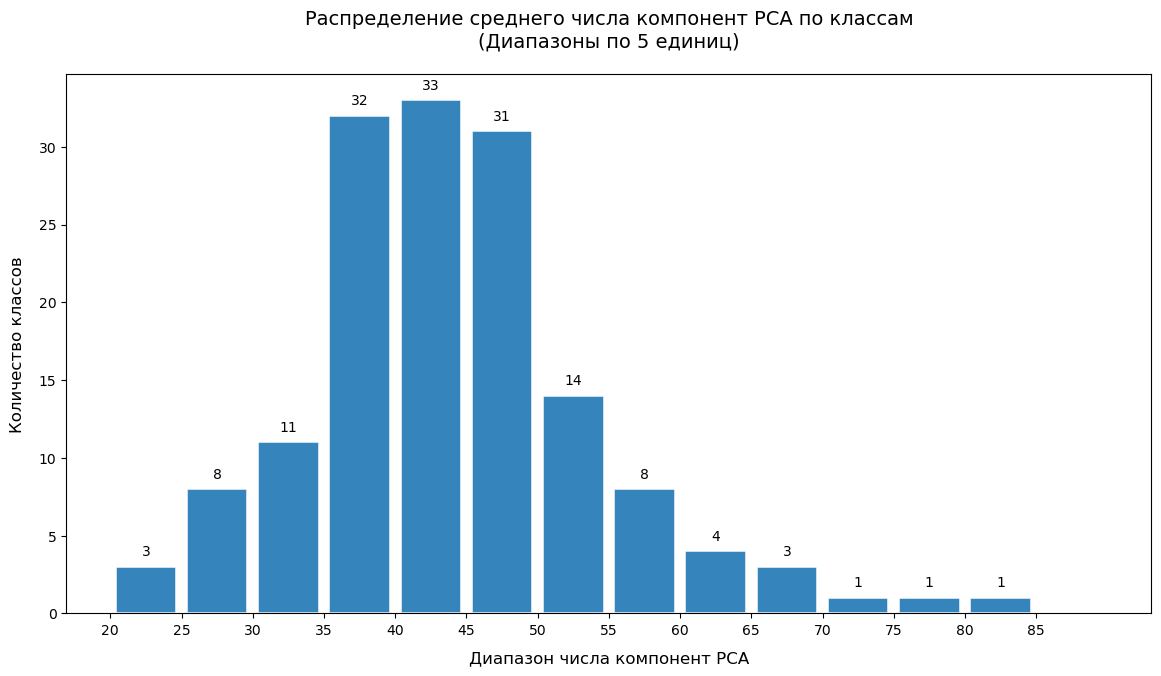
\includegraphics[width=0.8\textwidth]{components_by_class.png}
\caption{Распределение количества главных компонент по классам изображений.}
\label{fig:components_class}
\end{figure}

\begin{figure}[H] % Используем H для точного позиционирования
\centering
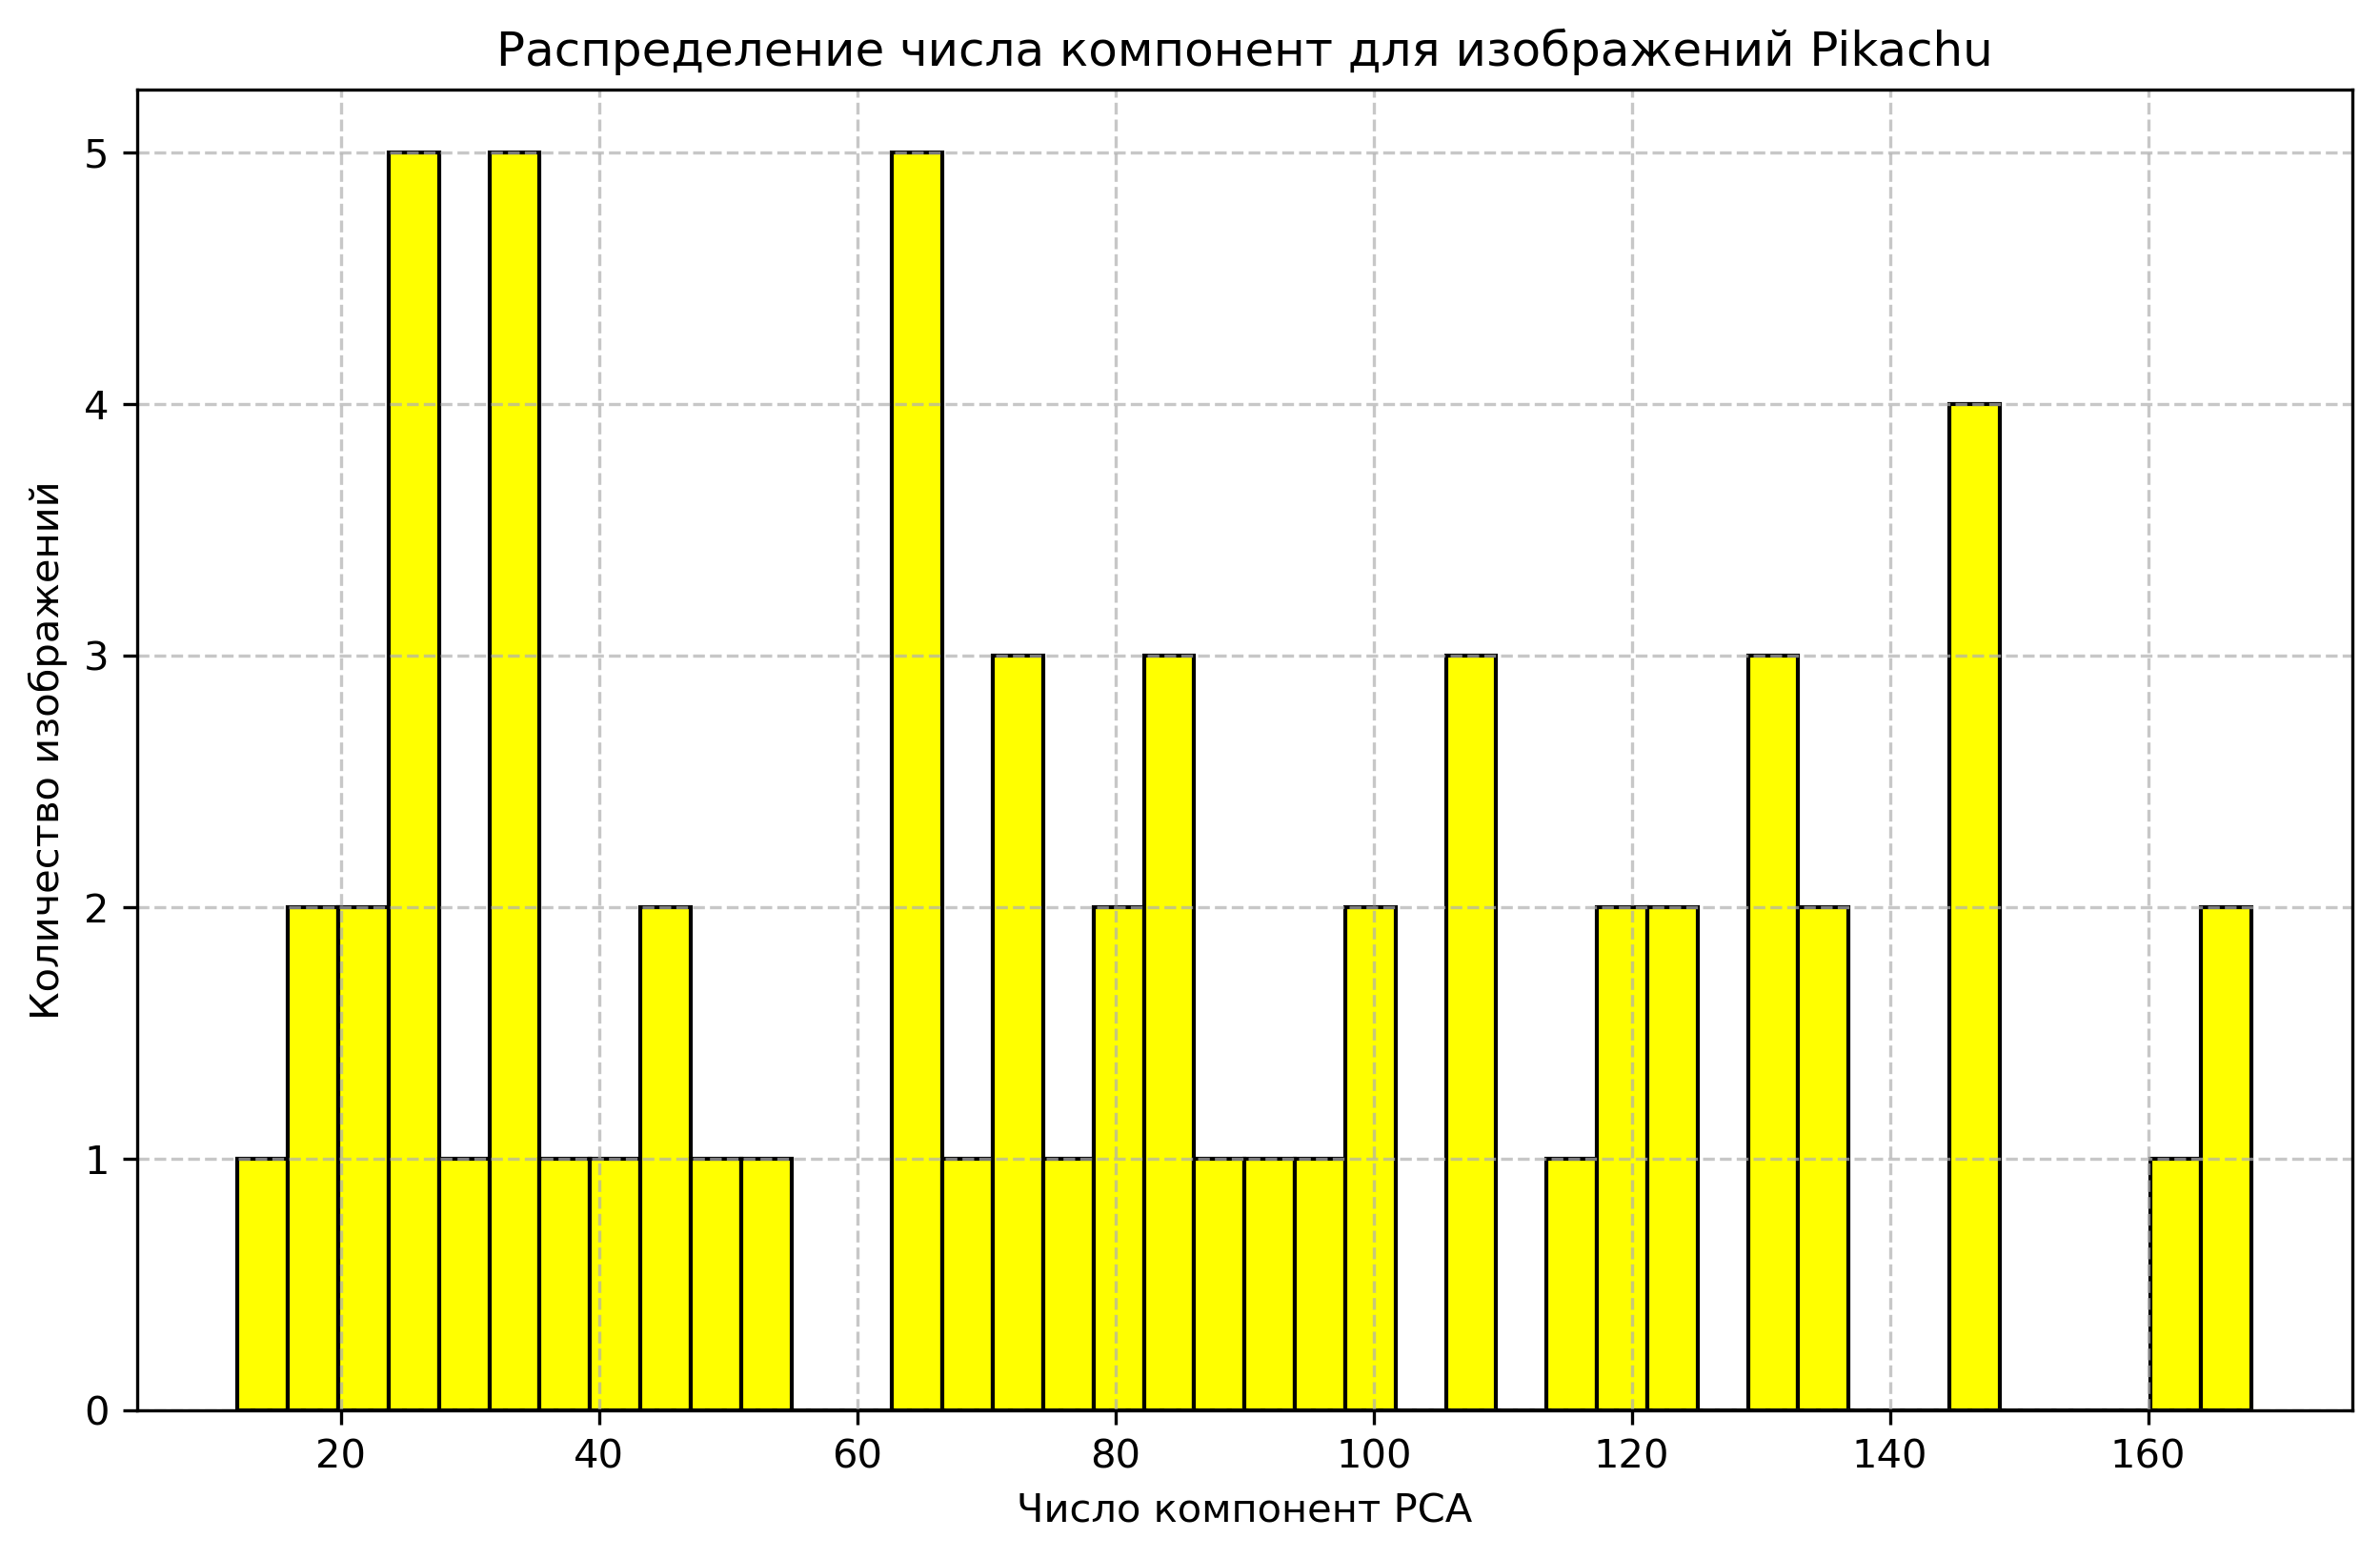
\includegraphics[width=0.8\textwidth]{components_by_image.png}
\caption{Вариация количества главных компонент для отдельных изображений внутри класса "Pikachu".}
\label{fig:components_image}
\end{figure}

\begin{figure}[H] % Используем H для точного позиционирования
\centering
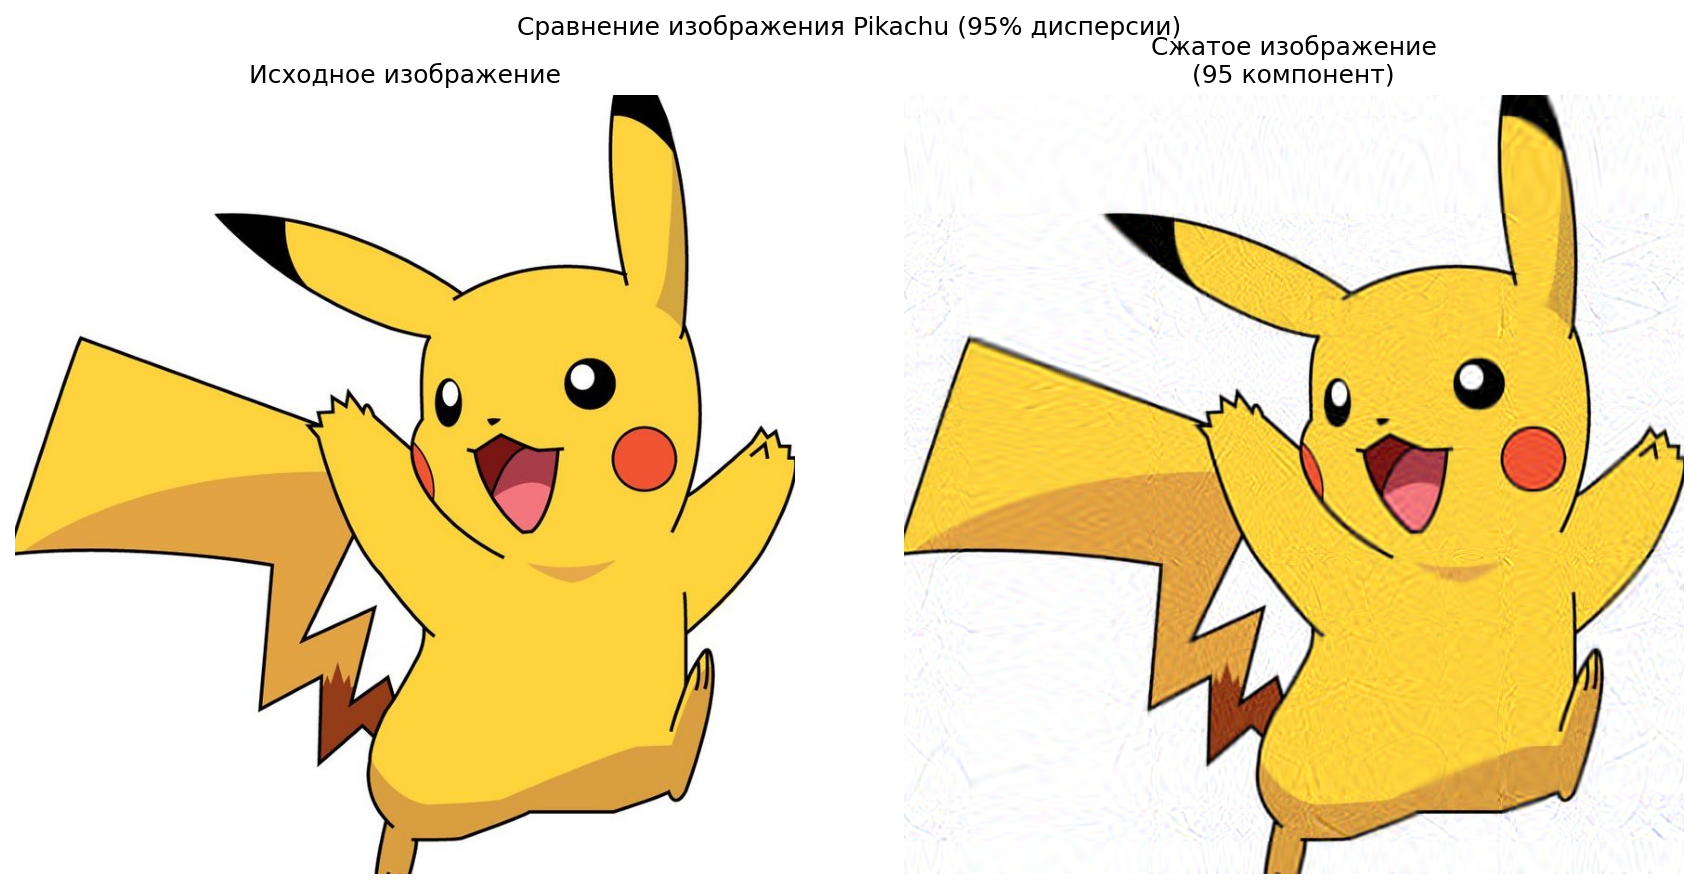
\includegraphics[width=0.8\textwidth]{pikachu_comparison.png}
\caption{Сравнение исходного и сжатого изображений класса "Pikachu".}
\label{fig:pikachu_comparison}
\end{figure}

\begin{table}[H]
\centering
\caption{Результаты сжатия изображений покемонов методом PCA}
\label{tab:compression_stats}
\resizebox{\textwidth}{!}{ % Автоматическое масштабирование по ширине
\begin{tabular}{@{}lrrr@{}} % @{} убирает лишние отступы
\toprule
Класс покемона & \begin{tabular}{@{}c@{}}Объём до\\сжатия (МБ)\end{tabular} & \begin{tabular}{@{}c@{}}Объём после\\сжатия (МБ)\end{tabular} & \begin{tabular}{@{}c@{}}Среднее число\\компонент\end{tabular} \\
\midrule
Abra & 37.72 & 16.42 & 39.54 \\
Aerodactyl & 19.18 & 10.70 & 36.69 \\
Alakazam & 23.06 & 12.52 & 40.65 \\
Alolan Sandslash & 26.87 & 17.19 & 48.34 \\
Arbok & 41.55 & 26.06 & 46.02 \\
Arcanine & 66.66 & 39.75 & 55.93 \\
Articuno & 48.90 & 46.61 & 70.31 \\
Beedrill & 21.40 & 15.35 & 44.82 \\
Bellsprout & 36.63 & 21.31 & 40.00 \\
Blastoise & 68.62 & 28.22 & 42.21 \\
\bottomrule
\end{tabular}
}
\end{table}


\section{Введение}

\subsection{Представление изображения в компьютере}
Цифровое изображение состоит из пикселей, где каждый пиксель кодируется интенсивностью трёх базовых цветов: красного (R), зелёного (G) и синего (B). Для примера рассмотрим изображение размером $2 \times 2$ пикселя:

\begin{equation*}
\begin{array}{ccc}
\text{Красный канал (R)} & \text{Зелёный канал (G)} & \text{Синий канал (B)} \\
\begin{bmatrix}
255 & 0 \\
0 & 255 \\
\end{bmatrix} &
\begin{bmatrix}
0 & 255 \\
0 & 255 \\
\end{bmatrix} &
\begin{bmatrix}
0 & 0 \\
255 & 255 \\
\end{bmatrix}
\end{array}
\end{equation*}

Здесь:
\begin{itemize}
\item Левый верхний пиксель: красный ($R=255$, $G=0$, $B=0$)
\item Правый верхний: зелёный ($R=0$, $G=255$, $B=0$)
\item Левый нижний: синий ($R=0$, $G=0$, $B=255$)
\item Правый нижний: белый ($R=255$, $G=255$, $B=255$)
\end{itemize}

\subsection{Метод главных компонент (PCA)}
Метод главных компонент (PCA) — это метод снижения размерности данных, который ищет ортогональный базис, максимизирующий дисперсию данных. PCA преобразует исходные данные в новые координаты, где первая главная компонента соответствует направлению наибольшей дисперсии, вторая — следующей наибольшей, и так далее. PCA находит ортогональный базис, где новые переменные (главные компоненты $pc_j$) линейно выражаются через исходные:

\begin{align*}
pc_1 &= v_{11} \cdot x_1 + v_{21} \cdot x_2 + \ldots + v_{k1} \cdot x_k \\
pc_2 &= v_{12} \cdot x_1 + v_{22} \cdot x_2 + \ldots + v_{k2} \cdot x_k \\
&\cdots \\
sCorr(pc_j, pc_n) &= 0 \quad \text{(ортогональность)} \\
\sum_{i=1}^k sVar(x_i) &= \sum_{i=1}^k sVar(pc_i) \quad \text{(сохранение дисперсии)}
\end{align*}

Для центрированных данных ($\bar{x}_j = 0$) главные компоненты вычисляются как:
\begin{equation*}
pc_j = X \cdot v_j \quad \text{и} \quad \|pc_j\|^2 = \lambda_j
\end{equation*}
где $\lambda_j$ — собственные числа, а $v_j$ — собственные векторы матрицы $X^T X$.

\subsection{Применение PCA для сжатия изображений}
Применяя PCA к каждой цветовой матрице изображения, можно сократить количество измерений, оставив только наиболее значимые компоненты. После преобразования изображение восстанавливается обратным проецированием главных компонент в исходный базис. Это позволяет уменьшить объём данных, сохраняя основную визуальную информацию.

\section{Ход работы}

В ходе исследования был выполнен следующий алгоритм обработки изображений покемонов:

\begin{enumerate}
\item \textbf{Загрузка изображений}: 
Использовались средства работы с файловой системой для рекурсивного обхода директорий и считывания изображений в форматах PNG и JPEG. Для каждого изображения сохранялась информация о классе покемона на основе структуры папок.

\item \textbf{Разложение на цветовые каналы}:
Каждое изображение разделялось на три матрицы, соответствующие интенсивности красного (R), зелёного (G) и синего (B) цветов (Рис.~\ref{fig:color_channels}). Это позволило анализировать цветовые компоненты независимо.

\item \textbf{Нормализация данных}:
Значения интенсивности приводились к диапазону [0, 1] путём деления на 255. Такая нормализация необходима для корректной работы алгоритма PCA и сравнения изображений разной яркости.

\begin{figure}[H]
\centering
\includegraphics[width=0.9\textwidth]{color_channels.png}
\caption{Пример разложения изображения Pikachu на цветовые каналы: (a) исходное изображение, (b) красный канал, (c) зелёный канал, (d) синий канал}
\label{fig:color_channels}
\end{figure}

\end{enumerate}


\section{Заключение}

В ходе выполнения данного проекта были достигнуты значительные результаты как в области освоения новых технологий, так и в практическом применении методов анализа данных. 

\subsection{Освоение технологий}
В процессе работы участницы проекта освоили работу с библиотеками компьютерного зрения \textbf{OpenCV} для обработки и анализа изображений, включая:
    \begin{itemize}
        \item Чтение и запись изображений в различных форматах
        \item Разделение цветных изображений на каналы (RGB)
        \item Преобразование цветовых пространств
    \end{itemize}

\subsection{Эффективность метода PCA}
Проведенные эксперименты показали, что метод главных компонент демонстрирует исключительную эффективность для задач сжатия изображений:
\begin{itemize}
    \item При сохранении \textbf{95\% объяснённой дисперсии} достигается сокращение:
    \begin{itemize}
        \item Объёма хранимых данных на \textbf{40\%}
        \item Количества признаков с \textbf{256 - 1120 до 12 - 167} главных компонент
    \end{itemize}
    
    \item Качество восстановленных изображений остаётся удовлетворительным для большинства практических применений
    
\end{itemize}

\subsection{Вычислительная сложность}
Несмотря на преимущества, метод имеет существенные ограничения:
\begin{itemize}
    \item Временная сложность полного PCA составляет $O(p^3 + np^2)$ для $n$ образцов размерности $p$
    
    \item Для изображений высокого разрешения (4K и более) требуются:
    \begin{itemize}
        \item Оптимизированные алгоритмы (Randomized PCA)
        \item Высокопроизводительные вычислительные ресурсы
        \item Использование GPU-ускорения через CUDA
    \end{itemize}
    
    \item Потребление памяти растёт квадратично с увеличением размерности данных
\end{itemize}
\subsection{Вывод}
Таким образом, проект продемонстрировал как практическую ценность метода PCA для обработки изображений, так и важность учёта вычислительных ограничений при работе с большими объёмами данных.

\end{document}